% EOR schematic -- corrected version
% Fixes vs. the original: duplicate "Natural Flow" -> Waterflooding / Immiscible gas injection,
% "Artifical" typo, gas / chemical / thermal / microbial labels completed, bypass arrow
% explained, brace-style brackets, descriptive caption.
\documentclass[tikz,border=10pt]{standalone}
\usepackage{lmodern}
\renewcommand{\familydefault}{\sfdefault}
\usepackage[T1]{fontenc}
\usepackage{amsmath}
\hyphenpenalty=10000 \exhyphenpenalty=10000
\usetikzlibrary{positioning,arrows.meta,calc,decorations.pathreplacing,backgrounds}

\definecolor{conv}{RGB}{70,110,170}
\definecolor{eor}{RGB}{200,100,40}

\begin{document}
	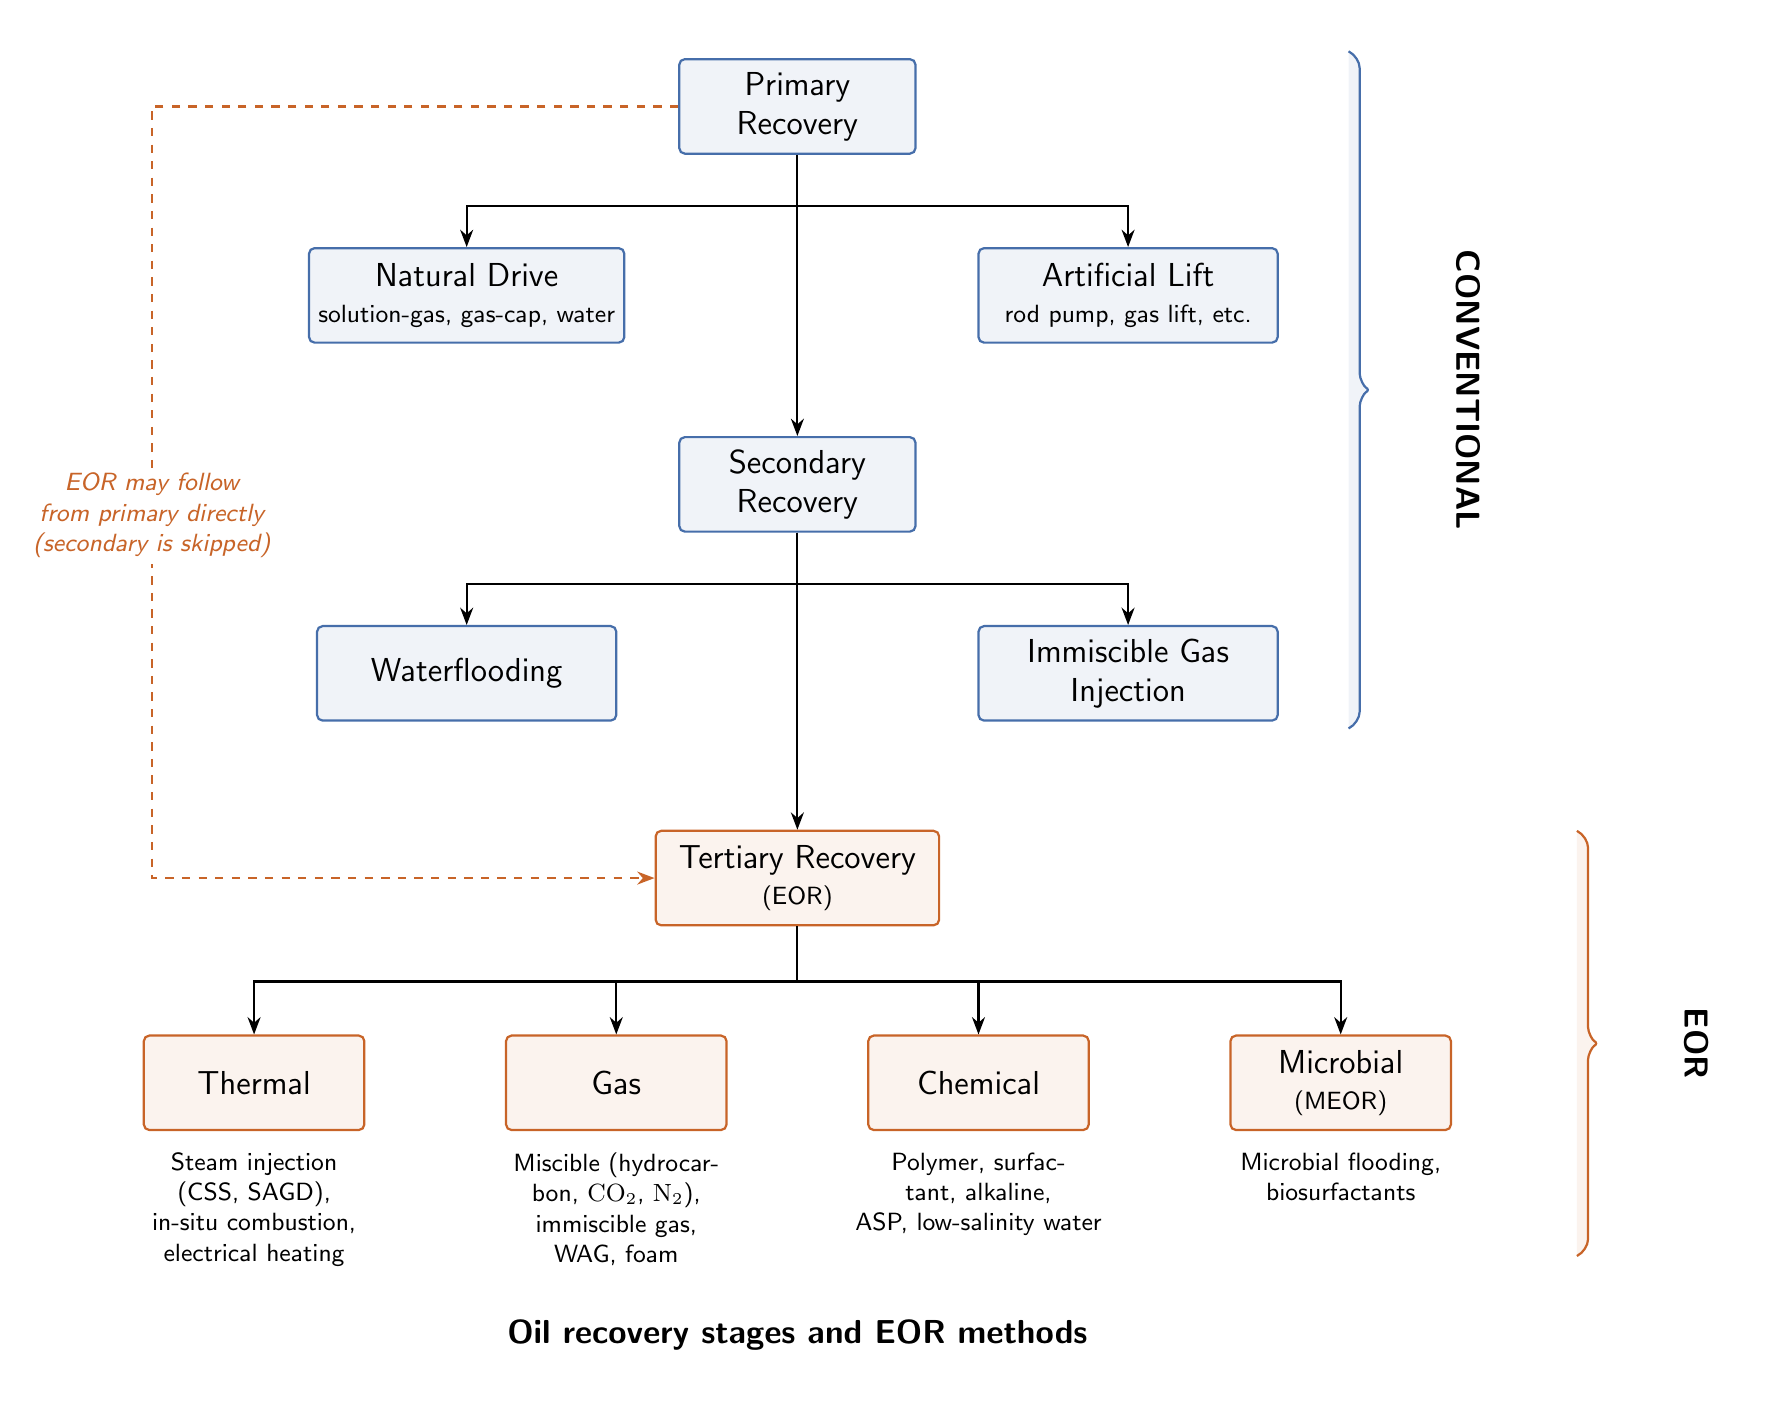
\begin{tikzpicture}[
		>={Stealth[length=2.2mm]},
		box/.style={draw, thick, rectangle, rounded corners=2pt, minimum width=3.0cm,
			minimum height=1.2cm, align=center, font=\large},
		conv/.style={box, draw=conv, fill=conv!8},
		eor/.style={box, draw=eor, fill=eor!8},
		note/.style={font=\small, align=center, text width=3.6cm, anchor=north},
		line/.style={thick}
		]
		% main stages
		\node[conv] (prim) at (0,0) {Primary\\Recovery};
		\node[conv, minimum width=3.8cm] (nf1) at (-4.2,-2.4) {Natural Drive\\[-1pt]{\small solution-gas, gas-cap, water}};
		\node[conv, minimum width=3.8cm] (al)  at (4.2,-2.4)  {Artificial Lift\\[-1pt]{\small rod pump, gas lift, etc.}};
		\node[conv] (sec) at (0,-4.8) {Secondary\\Recovery};
		\node[conv, minimum width=3.8cm] (nf2) at (-4.2,-7.2) {Waterflooding};
		\node[conv, minimum width=3.8cm] (pm)  at (4.2,-7.2)  {Immiscible Gas\\Injection};
		\node[eor, minimum width=3.6cm] (ter) at (0,-9.8) {Tertiary Recovery\\[-1pt]{\small (EOR)}};
		
		% EOR leaves
		\node[eor, minimum width=2.8cm] (th) at (-6.9,-12.4) {Thermal};
		\node[eor, minimum width=2.8cm] (ga) at (-2.3,-12.4) {Gas};
		\node[eor, minimum width=2.8cm] (ch) at (2.3,-12.4)  {Chemical};
		\node[eor, minimum width=2.8cm] (mi) at (6.9,-12.4)  {Microbial\\[-1pt]{\small (MEOR)}};
		\node[note] at ($(th.south)+(0,-0.15)$) {Steam injection (CSS, SAGD),\\ in-situ combustion,\\ electrical heating};
		\node[note] at ($(ga.south)+(0,-0.15)$) {Miscible (hydrocarbon, \ensuremath{\mathrm{CO_2}}, \ensuremath{\mathrm{N_2}}),\\ immiscible gas, WAG, foam};
		\node[note] at ($(ch.south)+(0,-0.15)$) {Polymer, surfactant, alkaline,\\ ASP, low-salinity water};
		\node[note] at ($(mi.south)+(0,-0.15)$) {Microbial flooding,\\ biosurfactants};
		
		% primary -> children
		\draw[line] (prim.south) -- ++(0,-0.65) coordinate (f1);
		\draw[line,->] (f1) -| (nf1.north);
		\draw[line,->] (f1) -| (al.north);
		\draw[line,->] (prim.south) -- (sec.north);
		% secondary -> children
		\draw[line] (sec.south) -- ++(0,-0.65) coordinate (f2);
		\draw[line,->] (f2) -| (nf2.north);
		\draw[line,->] (f2) -| (pm.north);
		\draw[line,->] (sec.south) -- (ter.north);
		% bypass: primary -> tertiary (EOR may follow primary directly)
		\draw[line,->,dashed,draw=eor] (prim.west) -- (-8.2,0) -- (-8.2,-9.8) -- (ter.west);
		\node[font=\small\itshape, text=eor, align=center, fill=white, inner sep=2pt]
		at (-8.2,-5.2) {EOR may follow\\from primary directly\\(secondary is skipped)};
		% tertiary -> leaves
		\draw[line] (ter.south) -- ++(0,-0.7) coordinate (f3);
		\foreach \n in {th,ga,ch,mi} \draw[line,->] (f3) -| (\n.north);
		
		% make sure braces are inside the bounding box
		\path (10.8,1.0) (-9.4,-16.2);
		% brace brackets
		\draw[decorate,decoration={brace,amplitude=8pt},thick,conv] (7.0,0.7) -- (7.0,-7.9)
		node[midway,xshift=0.9cm,rotate=-90,anchor=south,font=\large\bfseries] {CONVENTIONAL};
		\draw[decorate,decoration={brace,amplitude=8pt},thick,eor] (9.9,-9.2) -- (9.9,-14.6)
		node[midway,xshift=0.9cm,rotate=-90,anchor=south,font=\large\bfseries] {EOR};
		
		\node[font=\large\bfseries] at (0,-15.6)
		{Oil recovery stages and EOR methods};
	\end{tikzpicture}
\end{document}